\documentclass[11pt]{article}
\usepackage{times}
\usepackage{latexsym}
\usepackage{graphicx}
\usepackage{booktabs}
\usepackage{amsmath}
\usepackage{todonotes}
\usepackage{multirow}
\usepackage{enumitem}
\usepackage{amsfonts}
\usepackage{url}
\makeatletter
\newcommand{\@BIBLABEL}{\@emptybiblabel}
\newcommand{\@emptybiblabel}[1]{}
\makeatother
\usepackage[hidelinks]{hyperref}
\DeclareMathOperator*{\argmax}{arg\,max}
\newcommand*{\checktikz}[1][]{\tikz[x=1em, y=1em]\fill[#1] (0,.35) -- (.25,0) -- (1,.7) -- (.25,.15) -- cycle;}
\newcommand*{\crosstikz}[1][]{\tikz[x=1em, y=1em]\fill[#1] (0,0) -- (1,1) -- (0.5,0.5) -- (0.1,0.1) -- cycle;}


\newcommand{\Correct}{\checktikz[draw=black]}
\newcommand{\ValidMiss}{\checktikz[draw=gray,fill=white]}
\newcommand{\Valid}{\checktikz[draw=gray,fill=white]}
\newcommand{\Missed}{\checktikz[draw=black]} %\textsf{X}~}
\newcommand{\Wrong}{} %\textsf{X}~}

\newcommand{\U}{\mathbb{U}}

\begin{document}


\section{Abstract}

Asking questions is fundamental to communication, and machines cannot effectively collaborate with humans unless they can ask questions. Asking questions is also a natural way way for machines to express uncertainty, a task of increasing importance in an automated society. Despite decades of work on question answering, there is relatively little work in question asking.

\section{Introduction}

\subsection{Motivation}
https://www.skillsyouneed.com/ips/clarification.html
In communication, clarification involves offering back to the speaker the essential meaning, as understood by the listener, of what they have just said. Thereby checking that the listener's understanding is correct and resolving any areas of confusion or misunderstanding.

Clarification is important in many situations especially when what is being communicated is difficult in some way.

%Read more at: https://www.skillsyouneed.com/ips/clarification.html
%-- talk about difference between clarification questions and probing questions
%-- types of clarification questions: open & closed (http://study.com/academy/lesson/clarifying-questions-definition-examples.html)

\section{Related Work}

\subsection{Question Generation}

The problem of question generation has received sparse attention from the natural language processing community. Most prior work focuses on generating reading comprehension questions:  given text, write questions that one might find on a standardized test \cite{vanderwende2008importance,heilman2011automatic,rus2011question,olney2012question}.  Comprehension questions, by definition, are answerable from the provided text. Clarification questions are not.  

Outside reading comprehension questions, \cite{labutov2015deep} generate high-level question templates by crowdsourcing and given a text segment, rank question templates that are relevant. However the crowdsourcing method of collecting data leads to significantly less data than we collect using our method. \cite{liu2010automatic} use template question generation to help authors write better related work sections. \cite{mostafazadeh2016generating} introduce a Visual Question Generation task where they consider question generation from images, a multi-modal variant of question generation. 
\cite{penas2010filling} identify the notion of missing information similar to us but they attempt to fill the knowledge gaps in a text with the help of external knowledge bases, whereas we instead ask clarification questions. \cite{artzi2011bootstrapping} use human-generated clarification questions to drive a semantic parser where the clarification questions are aimed towards simplifying a user query; whereas we generate clarification questions aimed at  identifying missing information in a text. 

- Question generation shared task: http://www.aclweb.org/anthology/W11-2853

\subsection{Neural networks in NLP}

\subsection{Dialogue modeling}

Following the introduction of the Ubuntu dialogue dataset, there has been several recent work in modeling dialogue that uses this dataset. \cite{DBLP:conf/sigdial/LowePSP15} describe two neural network baseline models using Recurrent Neural Network (RNN) and Long Short Term Memory (LSTM). 
\cite{DBLP:journals/corr/KadlecSK15} create an ensemble of LSTMs, Bi-LSTMs and CNNs to get improved baselines. 
\cite{xu2016incorporating} incorporate domain knowledge by enhancing their LSTM model with a recall gate.
\cite{serban2016hierarchical} introduce a latent variable hierarchical recurrent encoder-decoder model by adding a context level RNN that processes sequences of sub-sequences operating on top of the token level RNN.
\cite{serban2016multiresolution} take a similar hierarchical approach but instead of defining a latent coarse representation, they assume it to be observed and experiment with two such representations (sequence of nouns and sequence of activities and entities).
\cite{baudivs2016sentence} introduce a unified approach for scoring sentence pairs applicable to number of tasks including next utterance classification and show best result on the Ubuntu dialogue corpus task. 

The techniques we combine in this work are best practices gleaned from the NLP modeling literature. 
The character trigram histogram technique (Section~\ref{character_level_modeling}) was introduced as word hashing \cite{DBLP:conf/cikm/HuangHGDAH13} to reduce the dimensionality of bag-of-words term vectors. Residual learning (Section~\ref{residual_learning}) was first introduced as a way to ease training of very deep networks in image recognition work \cite{he2015deep}. The technique of attention aggregation (Section~\ref{attention_aggregation} has been effectively used for several language based tasks like neural machine translation \cite{DBLP:journals/corr/BahdanauCB14}, \cite{DBLP:conf/emnlp/LuongPM15}, question answering \cite{} and others. More specifically in dialogue modeling, \cite{DBLP:journals/corr/YaoPZW16} have shown that attending to the context while generating the words of the response, similar to attention based model used for MT, gives an improvement over using just the last hidden state.

\section{Completed Work}

\subsection{Dialogue modeling}

\subsubsection{Main idea}

Data-driven methods for dialog have experienced a recent surge in
interest, due to a combination of the increasing availability of data and
improved machine learning techniques.  To facilitate public research,
\cite{DBLP:conf/sigdial/LowePSP15} put together the Ubuntu Dialogue
corpus by extracting two-way conversations from chat logs where people
were discussing about the issues they were having with the Ubuntu
Operating system.  

In this paper we describe several modifications to the reference model
which in combination achieve state of the art results on the Ubuntu
Dialog Corpus.  This is significant given the substantial attention that
this dataset has achieved in the literature.  Our modifications are
inspired by best practices in language modeling, and their simplicity
suggests general applicability for dialog modeling.  Succinctly, they
are: attention, character-level modeling, residual learning, and bursty
vocabulary selection.  Of these, only the last technique is novel, but
their combination on this dataset is highly effective and heretofore
unreported.

\subsubsection{Method description}\label{our_methods}

%\begin{figure}\label{sample_dialogue}
%\includegraphics[scale=0.35]{SampleContext}
%\includegraphics[scale=0.35]{SampleResponse}
%\caption{Example of a context and two responses to choose from \textbf{If we need space, this should be the first thing to go.}}
%\end{figure}

\begin{figure*}
\begin{tabular}{| c | l |}
\hline
Speaker & Utterances \\ \hline
0 & hmm, just mail me if you want \\ 
 & I'll follow the mail on the internal list \\ 
 & yes \\ \hline
 1 & gnome-setting-daemon is working! \\ \hline
 0 & Kamion has fixed it \\ \hline
 1 & everything still has .menu files right? \\
 & So installing the menu package and some hackery can get the Debian menu back? \\ \hline
 0 & no, we need a gnome-panel code change for this \\ \hline
 1 & ah, suck \\ \hline
 0 & the issue is ``we shouldadd .desktop file for the apps which need it ''  \\ \hline
 1 & = all packages providng user-runnable programs ? \\ \hline
\end{tabular}
\caption{Context of a conversation}
\label{sample_context}
\vspace{5mm}
\end{figure*}

\begin{figure*}
\begin{tabular}{| l | l |}
\hline
Actual response & that's a sensible question. We don't want to reacreate the mess of the debian menu... \\
& so not easy to know which app has its place in the menu or not :) \\ \hline
Random response & on xchat an uparrow will bring up the last thing you typed. \\
 & do it again and you get the previous one. \\
 & Wonderful device. So you can use xchat for irc and the other for gtalk \\ \hline
\end{tabular}
\caption{Two responses to choose from given the context above}
\label{sample_response}
\end{figure*}

\textbf{Dataset and baseline model}\\\\

The Ubuntu dialogue corpus is a collection of one million two
person conversations systematically extracted from the chat log
of forums discussing issues related to the ubuntu operating system.
The task associated with the dataset is next utterance classification,
which facilitates assessment while remaining plausibly related to more
complex design goals.  The problem given a portion of a conversation (Figure~\ref{sample_context}), and a set of possible next
responses (Figure~\ref{sample_response}), is to identify the correct next response.  The set of possible
next responses includes the true continuation of the conversation as well
as negative distractor utterances randomly sampled from the corpus.
\footnote{In version 2 of the corpus, the negative sampling is not
uniform, to increase the difficulty of identifying the next utterance.}

Several reference models are provided along with the dataset.  The best
reference model is our starting point: it is a siamese network of two
LSTMs, one for context and one for response, with tied weights. The
words of the context (and response) is fed into the LSTM one word at a
time. The final hidden state of the two LSTMs represents the summary of the
input context and the response respectively and the model is trained to
minimize the cross entropy of all labelled context, response pairs.

\textbf{Attention Aggregation}\label{attention_aggregation}\\\\

The baseline model described before uses the last hidden state of the LSTM
to represent the input. Our experiments indicate that a simple averaging
of the hidden states gives an improvement over using just the last state.
We achieve a further improvement with a simple attention mechanism.

The idea of attending to some part of the input more than the other was first used for translation \cite{DBLP:journals/corr/BahdanauCB14} where the probability of predicting a certain word on the target side was conditioned a distinct context on the source side. We use a similar notion of soft-attention by taking weighted average over the hidden states where the weights are learned during training. 

\textbf{Character level modeling}\label{character_level_modeling}\\\\

Most modeling of text for various NLP tasks have been done at the word
level. Recent work in neural machine translation has seen the benefit of modeling at a
sub-word level \cite{DBLP:conf/acl/Costa-JussaF16}. This can be especially
useful for natural dialog due to phenomena such as misspellings, elided
white spaces, and abbreviation.

We found character trigram histograms to be simple and highly effective.
Figure \ref{trigram_histogram} shows a sample trigram histogram of the
word \textit{bananas}. The left column lists all the trigrams in the
word and their frequencies.  Associated with each trigram is an index:
a trigram which occurs sufficiently frequently in the training corpus is
assigned a unique index, and all other trigrams are assigned the special
OOT index.  This defines a trigram frequency vector for any token.
This vector is then Hellinger transformed \cite{legendre2001ecologically} onto the unit sphere,
i.e., each count is square-rooted and then divided by the total count.

We concatenate the trigram histogram vector with the one-hot vector used
for a representing a word to get our final word vector.  This yields
two interesting properties.  First, the representations for two tail
tokens that have small edit distance will have larger inner product
than if the edit distance were large, facilitating statistical transfer
between tail terms of low edit distance.  Second, the use of dropout on
the input variables will facilitate statistical transfer between head
terms and tail terms with small edit distance, as the one-hot portion
of the representation will sometimes be dropped out.

\begin{figure}\label{trigram_histogram}
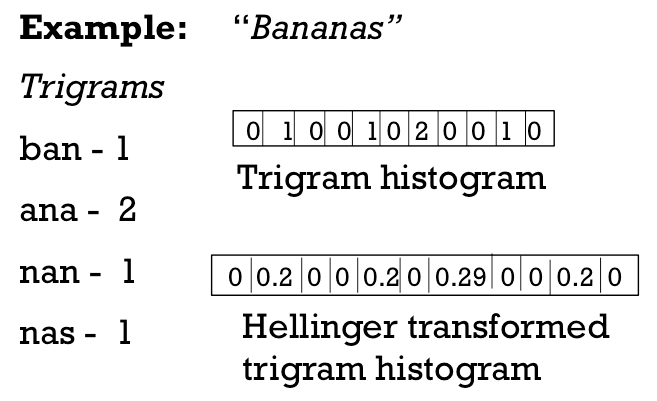
\includegraphics[scale=0.3]{TrigramHistogram}
\caption{Trigram histogram example}
\end{figure}

\textbf{Residual Learning} \label{residual_learning}\\\\

The idea of deep residual learning was first introduced by \cite{he2015deep} to ease the training of very deep neural networks. They observe that as network depth increases, training accuracy gets saturated and then degrades rapidly. To overcome this problem, they add shortcut connections between the stacked layers that perform mere identity mapping. They show that it is easier to optimize this residual mapping than to optimize the original, unreferenced mapping.

\textcolor{red}{Since our network does not have large number of layers, what was our motivation of using residual learning?}

\textbf{Bursty vocabulary}\\\\

Models that use vector representations for words often define the
vocabulary using a cutoff on the frequencies of words in the entire
corpus, replacing all lower frequency words with a special OOV token.
As is typical with power law statistics, there are a large number of
infrequently occuring tokens in the Ubuntu Dialogue corpus, e.g., due
to misspellings and incorrect tokenization.  Cross validation indicates
the optimal frequency cutoff for this dataset is actually quite high,
e.g., including tokens with a total count below 20 leads to overfitting.

However, these rare terms include tokens that are only used in a
few conversations, but which occur at a high frequency within 
these conversations.  Intuitively this could correspond to rare entities
that are the topic of a few conversations, and which would be 
highly discriminative for next utterance classification.

To safely induce a dedicated one-hot representation for such tokens
while avoiding overfitting, we define the following notion of a bursty
vocabulary: the frequency of a word is defined by its count in the
conversation where it occurs the most and a vocabulary is thereafter
defined using a cutoff on these word frequencies.  Experimentally
this simple approach is surprisingly effective.

To understand the idea of bursty vocabulary better, we inspected some
words from our corpus that were included in the bursty vocabulary and
excluded in the regular vocabulary and vice-versa. We call them bursty
non-frequent words and frequent non-bursty words respectively. Table
\ref{} shows the counts of these two categories of words. 

Some examples of bursty non-frequent words are \textit{`multicasting',
`techsupport',} and  \textit{`mutex'}.  When we looked at the
conversations where these words occurred the most we found that they
corresponded to conversations where the speakers were talking about an
issue with say multicasting, techsupport or mutex; these words were likely
to occur in the true next utterance but not in the distractor utterances.

On the other hand, some examples of frequent non-bursty words are
\textit{`insulting', `accurate'} and \textit{`baggage'}; suggesting that
words that generally occur a lot in the corpus may not be frequently
occurring within a conversation, and are therefore not useful for
identifying the true next utterance.


\subsection{Clarification Question Generation}

\subsubsection{Main idea}

A main goal of asking questions is to fill information gaps, typically through clarification questions, which naturally occur in conversations. 
A good question is one whose \emph{likely answer} is going to be most useful.
Consider the exchange in Figure~\ref{askubuntu_post}, in which an initial poster (who we'll call ``Terry'') asks for help configuring environment variables.
This question is underspecified and a responder (``Parker'') asks a clarifying question ``\textsf{\small (a) What version of Ubuntu do you have?}''
Parker could alternatively have asked one of:

\textsf{\small(b) Is the moon waxing or waning?}

\textsf{\small(c) Are you running Ubuntu 14.10 kernel 4.4.0-59-generic on an x86\_64 architecture?}

\noindent
Parker should not ask (b) because it's not useful; they should not ask (c) because it's too specific and an answer of ``No'' gives little help.
Parker's question (a) is optimal: it is both likely to be useful, and is plausibly answerable by Terry.
Our goal in this paper is is to automate Parker.
Specifically, after Terry writes their initial post, we aim to generate a clarification question so that Terry can immediately amend their post in hopes of getting faster and better replies.
\begin{figure}[!t]
\centering
\setlength\fboxsep{1pt}
\setlength\fboxrule{0.5pt}
\fbox{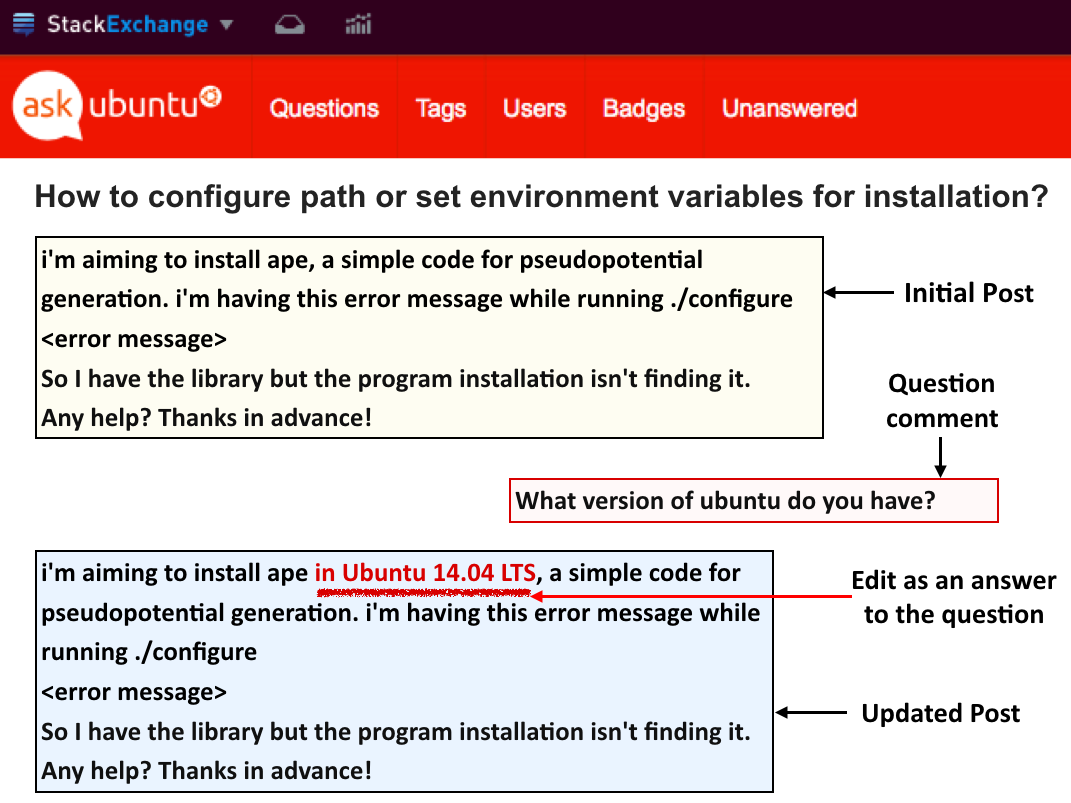
\includegraphics[width=0.47\textwidth]{askubuntu_post}}
\caption{A post on an online Q \& A forum ``askubuntu.com'' is updated to fill the missing information pointed out by the question comment}
\label{askubuntu_post}
\end{figure}
%
Our work has two main contributions: 
\begin{enumerate}[noitemsep,nolistsep]
%\item Identifying the problem of generating clarification questions as a problem worth of study, both in its own right and as part of the larger problem of building naturalistic conversational systems. 
\item A novel neural-network model for addressing this task that integrates the notion of expected value of perfect information (\S\ref{model}). % , a classic formalization from AI
\item A novel dataset, derived from StackExchange, that enables us to learn a model to ask clarifying questions by looking at the types of questions people ask (\S\ref{dataset_creation}).\footnote{We use data from StackExchange; per license cc-by-sa 3.0, the data is ``intended to be shared and remixed'' (with attribution). We will release all of the data we extract.}
\end{enumerate}

To develop our model we take inspiration from the decision theoretic framework of the Expected Value of Perfect Information (EVPI), a measure of the value of gathering additional information. In our setting, we use EVPI to calculate which question is most likely to elicit an answer that would make the post more informative.
Formally, for an input post $p$, we want to choose a question $q$ that maximizes $\mathbb{E}_{a \sim p,q}[\U(p+a)]$, where $a$ is a hypothetical answer and $U$ is a utility function measuring the \emph{completeness} of post $p$ if $a$ were to be added to it.
To achieve this, we construct two models:
(1) an answer model, which estimates $\mathbb{P}[a~|~p,q]$, the likelihood of receiving answer $a$ if one were to ask question $q$ on post $p$;
(2) a completeness model, $\U(p)$, which measures how complete a post is.
Given these two models, at prediction time we search over a shortlist of possible questions for that which maximizes the EVPI.

We are able to train these models jointly based on $(p,q,a)$ triples that we extract automatically from StackExchange.
Figure~\ref{askubuntu_post} depicts how we do this using StackExchange's edit history.  In the figure, the initial post fails to state what version of Ubuntu is being run. In response to Parker's question in the comments section, Terry, the author of the post, edits the post to answer Parker's clarification question. We extract the initial post as $p$, question posted in the comments section as $q$, and edit to the original post as answer $a$ to form our $(p,q,a)$ triples. 

Our results show significant improvements from using the EVPI formalism over both standard feedforward network architectures and bag-of-ngrams baselines, even when our system builds on strong information retrieval scaffolding. In comparison, without this scaffolding, the bag-of-ngrams model outperforms the feedforward network. We additionally analyze the difficulty of this task for non-expert humans, and give examples of system output. %on which our system does well, and several on which it does poorly.


\begin{figure*}[t]
\centering
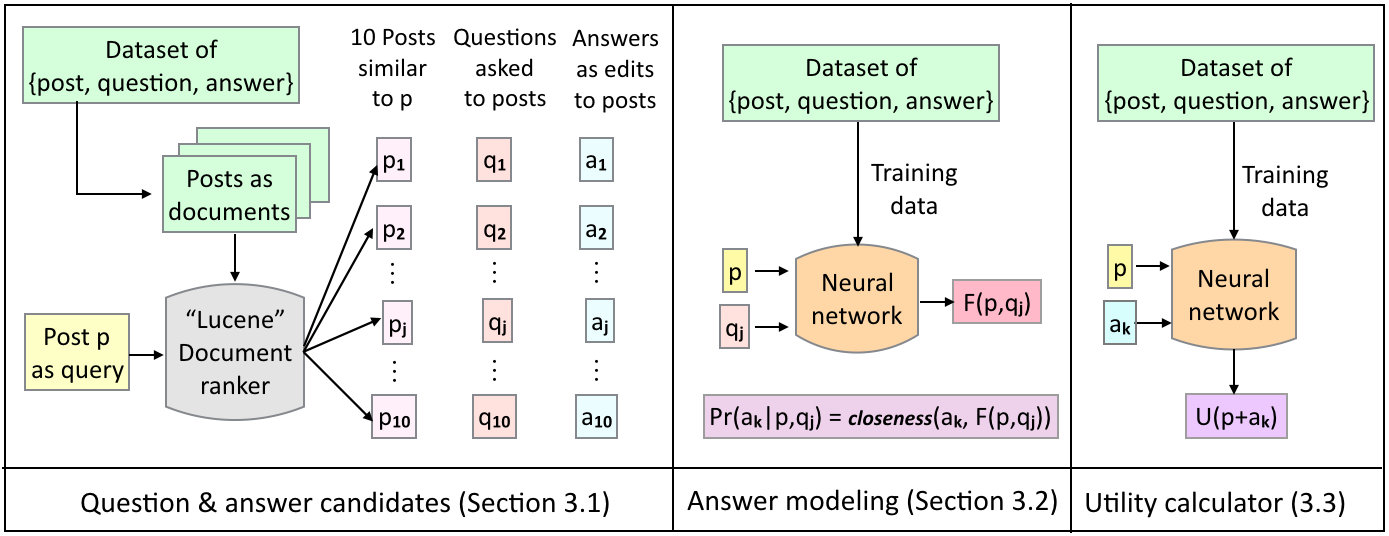
\includegraphics[width=0.85\textwidth]{model}
\caption{\small The behavior of our model during test time. Given a post $p$, Lucene retrieves 9 posts similar to post $p$ and consider the questions asked to those 9 posts, plus the original, as question candidates. The edits made to the posts in response to the questions as our answer candidates. For each question candidate $q_i$, we generate an answer representation $F(p,q_j)$ and calculate how close is the answer candidate $a_k$ to our answer representation $F(p,q_j)$. Our utility calculator calculates the utility of the post if it were updated with the answer $a_k$. Finally we return the question $q$ that maximizes the expected utility of the post $p$ (Equation~\ref{evpi_equation}).}
\label{model}
\end{figure*}


\subsubsection{Model description}\label{model}

In order to choose what question to ask, we build a neural network model inspired by the theory of expected value of perfect information (EVPI). EVPI is a measurement of: if I were to acquire information X, how useful would that be to me? However, because we haven't acquired X yet, we have to take this quantity in expectation over all possible X, weighted by each X's likelihood. In the question generation setting, for any given question $q$ that we can ask, there is set $A$ of possible answers that could be given. For each possible answer $a \in A$, there is some probability of getting that answer, and some utility if that were the answer we got. The value of this question $q$ is the expected utility, over all possible answers. The theory of EVPI then states that we want to choose the question $q$ that maximizes:
\begin{equation}\label{evpi_equation}
\argmax_{q \in Q} \sum_{a \in A} \mathbb{P}[a | p,q] \U(p+a)
\end{equation} 

In Eq~\ref{evpi_equation}, $p$ is the post, $q$ is a potential question from a set of candidate questions $Q$ and $a$ is a potential answer from a set of candidate questions $A$. $\mathbb{P}[a | p,q]$ measures the probability of getting an answer $a$ given an initial post $p$ and a clarifying question $q$. $\U(p+a)$ is a utility function that measures how useful it would be if $p$ were augmented with answer $a$. In our case, the utility function we use is the completeness of the post: a post has high utility the more complete it is. This captures the right intuition in the example questions (from Section~\ref{introduction}) that Parker could have asked such that: \textsf{\small (a)} will have good utility for many likely answers;
\textsf{\small (b)} will have low utility regardless of the answer; and
\textsf{\small (c)} will have high utility only for a low probability answer.

The modeling question then is how to model: 
%\begin{enumerate}[noitemsep,nolistsep]
(1) the probability distribution $\mathbb{P}[a | p,q]$ and
(2) the utility/completeness function $\U(p+a)$.
In our work, both will be represented using neural networks over the appropriate inputs. Posts, questions and answers will all be represented as embeddings. We train the parameters of the two models jointly to minimize a joint loss defined such that an answer that has a higher potential of increasing the utility of a post gets a higher probability.

Figure~\ref{model} describes the behavior of our model during test time. 
Given a post $p$, our first step is to generate a set of candidate questions and a set of candidate answers (Section~\ref{question_candidate_generator}).
Given a post $p$ and a question candidate $q_i$, our second step is to calculate how likely is this question to be answered using one of our answer candidates $a_k$ (Section~\ref{answer_modeling}).
Given a post $p$ and an answer candidate $a_k$, the third step is to calculate the utility of the updated post i.e. $\U(p + a_k)$ (Section~\ref{utility_calculator})
Finally, using these pieces, we build a joint neural network that we can optimize end-to-end over our data (Section~\ref{neural_network}).

\textbf{Question \& answer candidate generator}\label{question_candidate_generator}\\\\

Given a post $p$, our first step is to generate a set of candidate questions and a set of candidate answers. One way that humans learn to ask questions is by looking at how others ask questions in a similar situation. Using this intuition we generate question candidates for a given post by identifying posts similar to the given post and then looking at the questions asked to those posts. For identifying similar posts, we use Lucene\footnote{\url{https://lucene.apache.org/}}, a software extensively used in information retrieval for extracting documents relevant to a given query from a pool of documents. Lucene also ranks the extracted documents according to their relevance to the query. We use Lucene to find the top 10 most similar posts to a given post from our dataset (Section~\ref{dataset_creation}) \footnote{The top most similar candidate to a post is the original post itself}. We consider the questions asked to these 10 posts as our set of question candidates and the edits made to the posts in response to the questions as our set of answer candidates. Section~\ref{dataset_creation} describes the process of extracting the (\textit{post, question, answer}) triples from the StackExchange datadump. 

\begin{figure*}[ht]
\centering
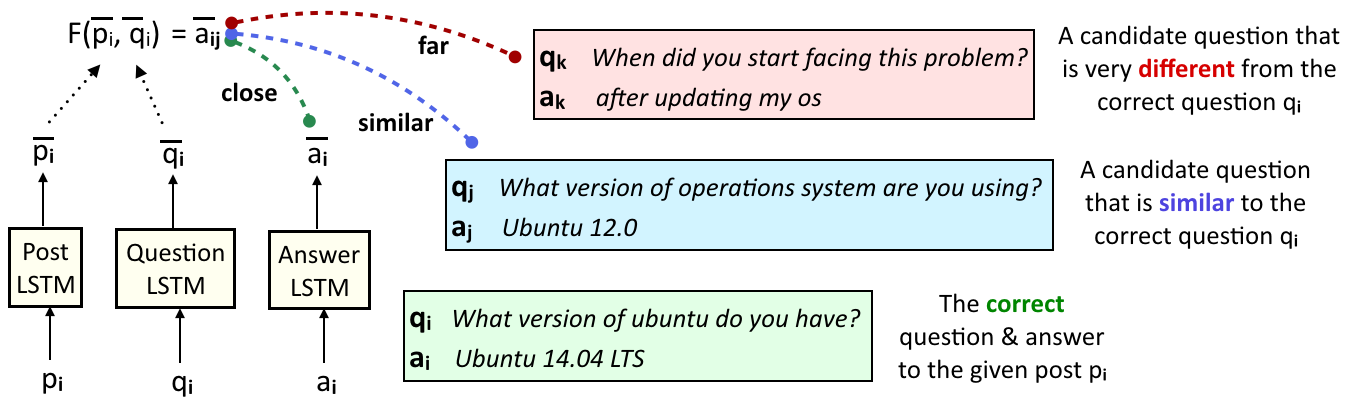
\includegraphics[width=0.9\textwidth]{answer_generator}
\caption{Training of our answer generator. Given a post $p_i$ and its question $q_i$, we generate an answer representation that is not only close to its correct answer $a_i$, but also close to one of its candidate answers $a_j$ if the candidate question $q_j$ is close to the true question $q_i$.}
\label{fig_answer_generator}
\end{figure*}

\textbf{Answer modeling}\label{answer_modeling}\\\\

Given a post $p$ and a question candidate $q_i$, our second step is to calculate how likely is this question to be answered using one of our answer candidates $a_k$. To calculate this probability, we first generate an answer representation using $p$ and $q_i$ and then measure how close is the answer candidate $a_k$ to our answer representation. To model our answer generator we use the following intuition: a question can be asked in several different ways. For e.g. in Figure~\ref{askubuntu_post}, the question ``\textsf{\small What version of Ubuntu do you have?}'' can be asked in other ways like ``\textsf{\small What version of operating system are you using?}'', ``\textsf{\small Version of OS?}", etc.  
Additionally, for a given post and a question, there can be several different answers to that question. For instance, ``\textsf{\small Ubuntu 14.04 LTS}", ``\textsf{\small Ubuntu 12.0}", ``\textsf{\small Ubuntu 9.0}", are all valid answers. We train our answer generator to generate an answer representation capturing these generalizations.

We use our dataset of \{\textit{post, question, answer}\} triples (Section~\ref{dataset_creation}). Given a $\{p_i, q_i, a_i\}$ triple, we use a long short-term memory architecture (LSTM) \cite{hochreiter1997long} to get to their respective neural hidden representations $\{\bar p_i, \bar q_i, \bar a_i\}$.  Given $(\bar p_i, \bar q_i)$, we define a feed-forward neural network $F$ that combines the post and question representations to get an answer representation $F(\bar p_i, \bar q_i)$. We train our answer generator to minimize the loss function below:
%
\begin{align}\label{eq_answer_generator}
  \textrm{loss}_{\textrm{ans}}(\bar p, \bar q, \bar a, Q) 
  &=  {|| F(\bar p, \bar q) - \bar a||}^2 & \\
  &\hspace{-25mm} +  \sum_{j \in Q} \Big ( {|| F(\bar p, \bar q) - \bar{a_j} ||}^2  (1 - \tanh{(|| \bar q - \bar{q_j} ||^2)}) \Big ) \Big \} &\nonumber
\end{align}
%
This loss function can be explained using the example in figure~\ref{fig_answer_generator}. Question $q_i$ is the question paired with the given post $p_i$. In equation~\ref{eq_answer_generator}, the first term forces the function $F(\bar p_i, \bar q_i)$ to generate an answer representation as close as possible to the correct answer $a_i$. Now, a question can be asked in several different ways. Let $Q_i$ be the set of candidate questions for post $p_i$, retrieved from the dataset using Lucene (Section~\ref{question_candidate_generator}). Suppose a question candidate $q_j$ is very similar to the correct question $q_i$ ( i.e. $|| \bar q_i - \bar{q_j} ||$ is near zero). Then the second term forces the answer representation $F(\bar p_i, \bar q_i)$ to be close to the answer $a_j$ corresponding to the question $q_j$ as well. Thus in the figure~\ref{fig_answer_generator}, the answer representation will be close to $a_j$ (since $q_j$ is similar to $q_i$), but far off from $a_k$ (since $q_k$ is dissimilar to $q_i$).

Given such an answer representation, we then define the probability distribution over candidate answers $a_k \in A$ as: 
\begin{align}
\mathbb{P}[a_k |p_i,q_j]  
&= \frac 1 Z \exp\left[- \lambda || a_k  -  F(p_i,q_j) ||^2\right]
\end{align}
where $\lambda$ is a tunable parameter that controls the variance of the distribution.

\textbf{Utility calculator}\label{utility_calculator}\\\\
Given a post $p$ and an answer candidate $a_k$, the third step is to calculate the utility of the updated post i.e. $\U(p + a_k)$. As expressed in equation~\ref{evpi_equation}, this utility function measures how useful it would be if a given post $p$ were augmented with an answer $a_k$. We train our utility calculator using our dataset of \{\textit{post, question, answer}\} triples (Section~\ref{dataset_creation}). We label all the $(p_i, a_i)$ pairs from our triples dataset with label $y=1$. To get negative samples, we make use of the answer candidates generated using Lucene as described in Section~\ref{question_candidate_generator}. For each $a_k \in A_i$, where $A_i$ is the set of answer candidates for post $p_i$, we label the pair $(p_i, a_k)$ with label $y=0$, except for when $a_k == a_i$. Thus, corresponding to each post $p_i$ in our triples dataset, we get one positive sample and nine negative samples. 

Given a post $p$ and an answer $a$, we use a post LSTM and an answer LSTM to get the neural representation $\bar{p}$ and $\bar{a}$. We define a feedforward neural network that combines the post neural representation $\bar{p}$ and the answer neural representation $\bar{a}$ to get the updated post representation $F(\bar{p}, \bar{a})$. The utility of the updated post is then defined as $\U(p+a) = \sigma ( F(\bar{p}, \bar{a}) )$. We want this utility to be close to 1 for all the positively labelled $(p,a)$ pairs and close to 0 for all the negatively labelled $(p, a)$ pairs. We therefore define our loss using the binary cross-entropy formulation below:
%
\begin{align}\label{eq_utility_calculator}
  \textrm{loss}_{\textrm{util}}(y, \bar p, \bar a) &= y \log(\sigma (F(\bar{p}, \bar{a})))
\end{align}

\textbf{Our joint neural network model}\label{neural_network}\\\\

Our fundamental representation is based on recurrent neural networks over word embeddings. We obtain the word embeddings using a GloVe \cite{pennington2014glove} model trained on the entire datadump of StackExchange. Given an initial post $p$, we generate a post neural representation $\bar{p}$ using a post LSTM i.e. long short-term memory architecture \cite{hochreiter1997long} as shown in the figure~\ref{lstm}. Similarly, given a question $q$ and an answer $a$, we generate a question neural representation $\bar{q}$ and a answer neural representation $\bar{a}$ using a question LSTM and an answer LSTM respectively. We define the function $F$ as a feedforward neural network on its input with two fully-connected hidden layers. So the function $F(\bar{p},\bar{q})$ in our answer model would be a feedforward neural network on the inputs $\bar{p}$ and $\bar{q}$ and the function $F(\bar{p}, \bar{a})$ in our utility calculator would be a feedforward neural network on the inputs $\bar{p}$ and $\bar{a}$. We train the parameters of the three LSTMs corresponding to $p$, $q$ and $a$, and the parameters of the two feedforward neural networks jointly to minimize the sum of the loss of our answer model (Eq~\ref{eq_answer_generator}) and our utility calculator (Eq~\ref{eq_utility_calculator}):
%
\begin{align}
                       \sum_i \textrm{loss}_{\textrm{ans}}(\bar p_i, \bar q_i, \bar a_i, Q_i)  
                        +  \textrm{loss}_{\textrm{util}}(y_i, \bar p_i, \bar a_i)
\end{align}
%
Given such an estimate $\mathbb{P}[a|p,q]$ of an answer and a utility $\U(p+a)$ of the updated post, predictions (i.e., selecting a question from a set of candidate questions) can be done by choosing that ``$q$'' that maximizes Eq~\ref{evpi_equation}. The remaining question, then, is how to get data that enables us to train our answer model and our utility calculator. Given data, the training becomes a multitask learning problem, where we learn simultaneously to predict utility and to estimate the probability of answers.

\begin{figure}
\centering
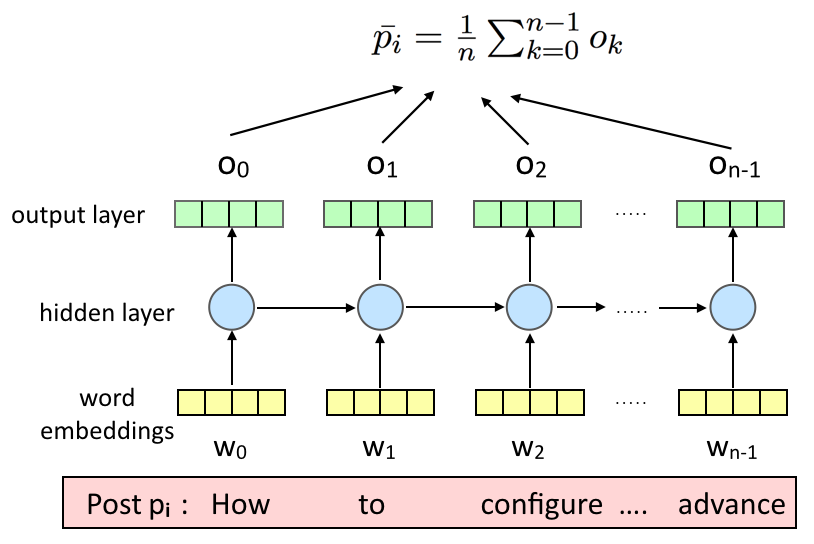
\includegraphics[scale=0.27]{lstm}
\caption{{\small Our LSTM architecture on a post $p_i$. The input layer consists of pre-trained word embeddings of the words in the post which is fed into a single hidden layer. The output $o_k$ of each of the hidden states is averaged together to get our neural representation $\bar p_i$}}
\label{lstm}
\end{figure}



\subsubsection{Dataset creation}\label{dataset_creation}
StackExchange is a network of online question answering websites about varied topics like academia, ubuntu operating system, latex, etc. The sites are modeled after StackOverflow, a popular platform used for asking and answering questions on a wide range of topics in computer programming. The data dump of StackExchange contains timestamped information about the posts, comments on the post and the history of the revisions made to the post. We use this data dump to create our dataset of \{\textit{post, question, answer}\} triples: where the \textit{post} is the initial unedited post, the \textit{question} is the comment containing a question and the \textit{answer} is the edit made to the post that matches the question comment. \\
\textbf{Extract posts:} We use the post histories to identify posts that have been updated by its author. We use the timestamp information to retrieve the initial unedited version of the post.\\
\textbf{Extract questions:} For each such initial version of the post, we use the timestamp information of its comments to identify the first comment made to the post. We look for a question mark `?' token to further identify if its a question comment. Finally, we truncate the comment till the question mark token to retrieve the question part of the comment.\\
\textbf{Extract answers:} In our final step, we identify the edit made to the post in response to the question comment. Authors make edits to their posts for several reasons; including stylistic updates and grammatical corrections. Therefore, we use only those edits that are longer than four words and finally use the timestamp information of the edit to match the edits to their respective question comments.

%We extract a total of 38,041 (\textit{post, question, answer}) triples from StackExchange which are distributed across three domains: askubuntu (13,749), unix (6656), and superuser (17,636). We train our models using 80\% of the data, tune our hyper parameters using 10\% of the data and evaluate our models using the remaining 10\% of the data. Table~\ref{data_statistics} shows the sizes of the train, dev and test splits for the three domains. 
\begin{table}
\centering
\begin{tabular}{lccc}
\toprule
& Train & Dev & Test  \\
\midrule
askubuntu & 10,992 & 1374 & 1375\\
unix & ~~~5324 & ~~666 & ~~666 \\
superuser & 14,828 & 1404 & 1404 \\
\bottomrule
\end{tabular}
\label{data_statistics}
\caption{Table above shows the sizes of the train, dev and test split of our dataset for three domains.}
\end{table}

A natural question to our process of data creation would be how often is the extracted question a clarification question. We sample a set of 1400 questions from our dataset and design a crowdsourced task where given a question we ask a human to choose whether: a) It is a clarification question, b) It provides an answer or a suggestion; or c) Neither.  63\% of the questions are marked as clarification question, 33\% of them are marked as questions that provides an answer or a suggestion and 4\% of them are marked as neither. The inter-annotator agreement (PAA) is above 90\%. These numbers suggest that although a greater percentage of the extracted questions are clarification questions, our data is imperfect: it includes some non-clarification questions.

\subsubsection{Experimental Results}\label{experiments_results}
Our primary research questions that we evaluate experimentally are:
%
\begin{enumerate}[noitemsep,nolistsep]
\item Does a neural architecture with learned representations improve upon a simple bag-of-ngrams baseline?

\item Does the expected value of perfect information (EVPI) formalism provide leverage over a similarly expressive feed-forward network? %In particular, is EVPI a useful inductive bias for a model?

\item In the EVPI formulation, is it useful to compute an expectation over answers, rather than just picking a single question/answer pair?

\item How well does our model perform in comparison to non-expert humans?

\item How much harder is the task when the (distrator) candidate questions come from Lucene rather than selected randomly?\footnote{A common strategy with the Ubuntu dialogue corpus \cite{lowe2015ubuntu} is to train a dialogue system by choosing a best response given a context of a conversation and a set of candidate responses. However, these methods generate their candidates from their dataset using random sampling. This plausibly makes the task significantly easier than using Lucene to select candidates, which are much more likely to be confusable and have high lexical overlap.}
\end{enumerate}

% In contrast, we generate our candidates using Lucene, a well-known information retrieval system, and so our candidate questions are more closer to each other than a randomly sampled questions would have been. Thus, we indirectly define a harder task. To compare how our models perform in an easier configuration, we design our experiments on two task setups (Section~\ref{task_setup}). To understand the leverage our EVPI inspired model gets us, we compare our model with non-neural baselines and feedforward neural baselines (Section~\ref{baselines}). 

% Further, we design another experiment where in equation~\ref{evpi_equation}, instead of choosing the question that maximizes the expected utility over all possible answers (EVPI max), we choose the question whose answer has the maximum utility (EVPI sum). This experiment helps us understand the leverage we are getting by summing over all our answer candidates, further strengthening the case for our EVPI inspired model. 

\begin{table*}[t]
\small
\centering
\begin{tabular}{l|cccc|cccc}
\toprule
 & \multicolumn{4}{c|}{Lucene negative candidates} & \multicolumn{4}{c}{Random negative candidates} \\
Models & Acc & MRR & R@3 & R@5 & Acc & MRR & R@3 & R@5\\
\midrule
Random  & 10.0 & 29.3 & 30.0 & 50.0 &10.0 & 29.3 & 30.0 & 50.0 \\
Bag-of-ngrams & 11.6 & 31.3 & 32.5 & 54.6 & 54.9 & 70.5 & 83.1 & 92.0 \\
Feed-forward & 17.4 & 37.8 & 43.2 & 63.9 &  49.0 & 66.8 & 81.3 & 92.8 \\
EVPI max  & 21.1 & 41.2 & 48.0 & 66.9  & 48.8 & 65.5 & 77.2 & 89.9 \\
EVPI sum & \bf 23.3 & \bf 43.4 & \bf 51.0 & \bf 70.3 & \bf 61.1 & \bf 75.5 & \bf 87.9  & \bf 95.8  \\
\bottomrule
\end{tabular}
\label{results_topN}
\caption{Results of our two setups `Lucene negative candidates' and `Random negative candidates' on askubuntu test split when the model is trained on a combination of askubuntu, unix and superuser train splits}
\end{table*}


\textbf{Task setups}\label{task_setup}\\\\

\textbf{Lucene negative candidates:} In this setup, given a post $p$, we label the question $q$ paired with $p$ in our dataset of $(p, q, a)$ triples as positive. To get our negative candidates, we retrieve nine additional question candidates using Lucene (as described in Section~\ref{question_candidate_generator}).\\
\textbf{Random negative candidates:} In this setup, given a post $p$, we label the question $q$ paired with $p$ in our dataset of $(p, q, a)$ triples as positive as in the previous setting. To get our negative candidates, we randomly sample nine other questions from our dataset of $(p, q, a)$ triples.\footnote{In all cases we train 100-d word embeddings using GloVe \cite{pennington2014glove} on the 3 billion token datadump of StackExchange. We use a threshold frequency of 100 to create our vocabulary of ~250,000 tokens. For our feed-forward neural network, we use two fully-connected dense hidden layers each of size 100. We use ReLU \cite{nair2010rectified} non-linearity as our activation function between the hidden layers.}


\textbf{Baseline methods}\label{baselines}\\\\

We compare our model with the following baselines:\\
\textbf{Random baseline:} Given a post, we randomly permute its set of 10 candidate questions uniformly.\\
\textbf{Bag-of-ngrams baseline:} Given a post and a set of 10 question question and answer candidates, we construct a bag-of-ngrams representation for the post, the question and the answer. Our bag-of-ngrams baseline is then trained to minimize hinge loss on misclassification loss using cross-product features between each of (\textit{post, question}), (\textit{question, answer}) and (\textit{post, answer}). We tune the ngram length and the learning rate and choose the setting that performs best on development data.\\
\textbf{Neural network baseline using post, question and answer:} We concatenate the post LSTM representation, the question LSTM representation and the answer LSTM representation and feed it through a feed forward neural network of two fully-connected hidden layers to get our neural baseline. 

\textbf{Dataset}\label{dataset}\\\\
We evaluate our model and our baselines on the following three domains of StackExchange: askubuntu, unix and superuser.
% \begin{description}
% \item[askubuntu:]  A question and answer site for users of the Ubuntu Operating system where people post queries about issues they face while using Ubuntu. An example question on this site: ``\textsf{\small Why isn't Chromium up-to-date in all the Ubuntu LTS repos, like Firefox is?}''
% \item[unix:]  A question and answer site for users of Linux, FreeBSD and other unix-like operating systems. This site would contain questions like the ones in askubuntu and more. An example question on this site: ``\textsf{\small How to repeatedly alternate between two (or more) commands?}''
% \item[superuser:] A question and answer site for users of all kinds of operating systems and computer applications. An example question on this site: ``\textsf{\small What is the LAST version of Windows Operating system that can run DOS applications natively?}''
% \end{description}
%
Table~\ref{data_statistics} shows the data statistics for the four sites above.  Although StackExchange consists of many sites, we choose the ones above because: a) The data dump available for them were moderately big in size to train a model on; b) These domains contain clarifications questions that are generic enough to be useful for many different posts; and finally c) The three domains were close enough so that we could combine them to create our full dataset of ~37K triples.

%\subsection{Experimental details}

%\paragraph{Preprocessing:} Each post, question and answer in our dataset of $(post, question, answer)$ triples is represented using embeddings. To generate these embeddings, we first tokenize the raw text in our post, question and answer. We restrict our post to be just the first 100 tokens of the post and our question and answer to be first 10 of their tokens respectively. Given these tokens we then use our word embeddings model to generate their embeddings.

%\paragraph{Word embedding model:} We train 100 dimensional word embeddings using GloVe \cite{pennington2014glove} on the 3 billion token datadump of StackExchange. We use a threshold frequency of 100 to create our vocabulary of ~250,000 tokens. 
%We then train a GloVe model on the datadump to get embeddings of size 100 for each token in our vocabulary. All tokens with a frequency of less than 100 in our dataset get assigned an `UNK'  token.

%\paragraph{Model hyperparameters:}  For our feed-forward neural network, we use two fully-connected dense hidden layers each of size 100. We use ReLU \cite{nair2010rectified} non-linearity as our activation function between the hidden layers. 

\textbf{Results}\\\\

We first describe results on the union of all data, summarized in Table~\ref{results_topN}.
We report four metrics: accuracy (percent of time the top ranked question was correct),
mean reciprocal rank (the reciprocal of the ranked position in the top ten list that the correct question is), 
recall at 3 (percent of the the correct answer is in the top three) and
at 5.

The left half of this table shows results when the candidate sets is from Lucene---the ``hard'' setting.
Here, we see that for all the evaluation metrics:
EVPI using the sum (expectation over $a$) outperforms
EVPI using the max $a$;
which outperforms the neural feedforward model that does not incorporate the EVPI formalism;
which outperforms the bag-of-ngrams baseline;
which outperforms the random baseline.
The gains in all cases are relatively large: at least a few percentage points.
A final performance of 51\% recall at 3 is encouraging, though clearly there is a long way to go for a perfect system.

The right half of this table shows the same results when the candidate set is chosen randomly---the ``easy'' setting.
A major difference in the results here is that the bag-of-ngrams system now \emph{outperforms} both the feedforward neural model and the EVPI using max instead of expectation.
This likely happens because just picking up on word overlap---when Lucene has not already done this for us---works remarkably well.
Nonetheless, in all of the metrics, the true EVPI model outperforms all the baselines, achieving at least a 3\% gain over the bag-of-ngrams baseline.

In Table~\ref{results_topM} (supplementary materials), we show results when we work not with the union of all the data, but with each data set individually.
%The top half is against Lucene candidate, the bottom half is against random candidates.
The main observation is that the trends are essentially the same as before: for Lucene negative candidates, bag-of-ngrams underperforms feedfoward, which underperforms EVPI.
This happens because more data helps, and these three domains are sufficiently similar that the additional data---even if it is slightly domain mismatched---is better than nothing.
%The second observation is that the results for EVPI are lower across the board, with the exception of superuser on random negative examples.% (which is sometimes better, sometimes worse).

\textbf{How well can humans do this task?}\\\\

In this section we address two natural questions:
(1) how does the performance of our system compare to a human solving the same task?
(2) just because the system selects a question that is not the exact gold standard question, is it certainly wrong?
To answer these questions, we had 14 computer science graduate students perform an annotation task on $50$ examples.
Most of these graduate students are \emph{not} experts in unix or ubuntu, but all are knowledgable.
We provided them with a post and a randomized list of ten possible questions.
They were instructed to select what they thought was the \emph{single} best question to ask, and additionally mark as ``valid'' any additional questions that they thought would also be okay to ask.
We also asked annotators to rate their confidence in $\{0,1,2,3\}$.
Most found this task quite challenging because many of the questions are about subtle nuances of operating system behavior.

These annotator's accuracy on the ``hard'' task of Lucene-selected questions, was only 36\%, significantly better than our best system (23\%), but still far from perfect.
If we limited to those examples on which they were more confident (confidence of 2 or 3), their accuracy raised to 42\%, but never surpassed that.
A major problem for the human annotators is the amount of background knowledge required to solve this problem.
On an easier domain, or with annotators who are truly experts, we might expect these numbers to be higher.

The average number of ``valid'' answers for a single post according to the (admittedly non-expert) annotators was 4.26 (out of ten); the distribution was fairly symmetric and quickly decaying around that number (the median is four).
In the data, 56\% of the examples had at most four options marked as valid; 
28\% had at most 3; 14\% had at most 2; and 6\% had only one valid option (which by definition is also the ``best'' option).
These numbers suggest that an evaluation strategy that takes validity---and not just raw accuracy---is a useful avenue for future research.

\textbf{Example Outputs}\\\\

To understand the behavior of the model, we have included five example outputs as supplementary material.
Table~\ref{tab:examples_good} shows two examples in which our model succeeds in selecting the correct question.
In the first, the original poster is asking a question about SSD data and hardware.
The model correctly asks about uefi (the Unified Extensible Firmware Interface, which replaces BIOS), and ranks that output significantly higher than its second guess.
This is particularly impressive since the question mentions neither uefi nor bios. Human annotators said that the third and fifth outputs would also be valid. In the second example, a user is having significant difficulty getting their Ubuntu installation to work, and the model correctly asks about the error of \texttt{\small apt-get install}.
Several other options were marked as valid by annotators in this case as well.

Table~\ref{tab:examples_bad} shows three examples of errors.
In the first example (about sound), the model
completely misses (ranks in last place) the true question about \texttt{\small linux-firmware-nonfree}.
The model instead asks about Pulseaudio, considered a valid question by annotators.
In the second example, the truth is about \texttt{\small apt-get update} but the model instead asked for the ubuntu version (generally a safe bet, and considered valid). %In this case the model fared better and put the correct question in second position.
In the third example, the model asks far too specific a question about \texttt{\small sslstrip-0.9.tar.gz}, rather than the more debugging question which it should have asked about (in position two).
In this case, it's guess was invalid.


\subsubsection{Conclusion}

We have described a new dataset for question generation, and attacked this problem from the perspective of question selection.
Our model integrates state-of-the-art neural network structure with the classic notion of expected value of perfect information, which effectively models a pragmatic choice on the part of the questioner: how do I \emph{imagine} the other party would answer if I were to ask this question. Such pragmatic priciples have recently been shown to be useful in other tasks as well \cite{golland2010game,smith2013learning,orita2015discourse,andreas2016reasoning}.

There are three main avenues for improvement of this work.
The first is in evaluation: given that this task is so difficult for humans, but also given that there is no single right question to ask, how can we better measure performance at this task?
This is exactly the same question faced in much research in dialog and generation more broadly \cite{paek2001empirical,lowe2015ubuntu,liu2016not,kannan2017adversarial}.
Second, to make question generation more general, systems need to be able to generalize, for instance by constructing templates of the from ``What version of \_\_\_ are you running?'' into which the system would need to fill a variable. Finally, asking question is a natural component of dialog, and building a collaborative dialog system that can naturally converse with a user is a broad long term goal.

\section{Proposed Work}

\subsection{Generating question templates}

In our preliminary work, we focused on building a model that can learn to select a question to ask from a candidate set of prior questions. To make the system more general, it needs to be able to generalize to new context well. Therefore, in this work, we propose to generate templates for questions. For e.g. consider a template like ``What version of \_\_\_  are you running?''. This template can generate thousands of specific variants found in the data like ``What version of Ubuntu are you running?'', ``What version of OS are you running?'', ``What version of apt-get are you running?'', etc. We identify four components to this template form of question generation:
\begin{enumerate}
\item Identifying near similar questions from a huge collection of questions
\item Identifying topic specific words in the questions and removing them to generate templates
\item Given a post, selecting the right question template from a candidate set of question templates
\item Filling in the blanks in the template using relevant context from the given post.
\end{enumerate}

\subsubsection{Background}
 Template generation is well studied in question answering (Ravichandran \& Hovy, 2002) and information extraction (Riloff, 1996), but not for question generation.

\subsubsection{Identifying similar questions}

We propose two strategies for identifying similar questions:

\textbf{Using clustering algorithm}: Given a set of clarification questions, we first use clustering algorithm (explore all available clustering algorithms) and cluster questions - Look at the cluster outputs. If they don't look useful, then use the next strategy - Can we remove topic specific words from questions to make them general? And then use clustering algorithm.

\textbf{Using Lucene}: Given a question, we use Lucene to identify top N questions similar to the given question. Do this for each question and then create question clusters from this information.

\subsubsection{Extracting templates}

Given a set of questions that are near similar, the next step is to extract a generic template which can be expanded to (almost) each of the variants in the set. We use the parts-of-speech information of the words in the question to identify proper nouns (and others) that indicate specific topics. Given these markings, we remove them from the questions to generate a template. Further, we classify questions into probable question types using an idea similar to \cite{}.

%- We can use POS tags to identify proper nouns (and others) which indicate specific words
%- Extracting patterns from text: https://www.cs.utah.edu/~riloff/pdfs/aaai96.pdf
%- Clustering questions: http://nlp.stanford.edu/courses/cs224n/2007/fp/paranjpe.pdf -- use POS tags to extract topic of a question (neat idea) --- classify questions in question types
%- Generating question templates using (query -> QA website question) pairs - http://www.aclweb.org/anthology/I11-1104 (poorly written :/) - related work is very exhaustive!

\subsubsection{Selecting question templates at test time}

Given a post, the next step then is to generate a set of candidate question templates and then to select the most relevant question template from the set of candidates. We use our previous model for this step.

\subsubsection{Filling in the blanks in the templates}

- How do we do this? Talk to Hal

\subsection{Generating questions using neural network generative model}

\begin{enumerate}
\item Person based dialog modeling: https://arxiv.org/pdf/1603.06155.pdf
\item Sequence to sequence model: https://papers.nips.cc/paper/5346-sequence-to-sequence-learning-with-neural-networks.pdf
\item Neural network generative question answering model: https://arxiv.org/pdf/1512.01337.pdf  -- their answer model inquires a knowledge base to retrieve the answer. The answer language model decides, at each time step, whether to generate a common vocabulary word or a knowledge base answer word
\item Idea: Seq2Seq model for generating a clarification question given context of the post
\item Blog on dialog progress: http://www.wildml.com/2016/04/deep-learning-for-chatbots-part-1-introduction/  
\end{enumerate}

\subsection{Clarification question for multi-turn dialogues}

\begin{enumerate}
\item Clarification questions for spoken dialogue systems  -- the focus here is more on generating naturally occuring clarification questions i.e. questions that are more context specific as opposed to saying ‘please repeat’ like generic question %http://www.cs.columbia.edu/speech/PaperFiles/2014/AISB2014_StoyanchevLiuHirschberg_final.pdf
\item Clarifying the specific entity in the text (more like word sense disambiguation): % https://pdfs.semanticscholar.org/eb75/46bdc723bc07c24c66a05b34ab264b4c7a0c.pdf
 -- they use 3 approaches: type based (orange the fruit or orange the color), example based (state an e.g. to clarify) and usage based (state a usage to clarify). They designed rules to extract such information from a large corpus
\item Clarifications questions for intention detection in language - % http://publications.eppe.eu/Trott_etal_Language_Intention_Ro-Man2016.pdf 
--  prior work section contains a lot of work related to us -- 
\item Clarification questions by a robot during human-robot dialogue - % http://cs.brown.edu/~stefie10/publications/deits13.pdf 
\item Idea: We extend our work on stackexchange by modeling multi-turn clarification questions in dialogues? Where we try to resolve some uncertainty by asking questions in multiple rounds. 
\item Concerns: dataset? Evaluation? Maybe we can extract questions from ubuntu dialogue corpus (or other corpus from IMDB like sitcoms (friends, big bang theory), OR twitter dialogues (recent msr paper on dialogue uses such datasets)
\end{enumerate}

\subsection{Information augmentation}
\begin{enumerate}
\item We define information augmentation as enhancing a given text with additional useful information. 
\item The goal is the following: given a fragment of text (paragraph or document), identify what information is structurally missing from the text. 
\item Rhetorical Structure theory (RST) gives us the structure of a paragraph in term of identify the nucleus ( main argument) and the satellites (supporting arguments) and also defines relations between them. -- Intro to RST: http://www.sfu.ca/rst/01intro/intro.html
\item We define our concrete task as follows: Given a paragraph, say we remove a sentence from the paragraph. The task is given a paragraph (with one of its sentences removed), its RST and given a set of candidate sentences (one of which is the true sentence), identify which sentence when added to the paragraph would add the missing information.
\item We approach this problem as follows: We take inspiration from Recursive Neural Networks which makes use of the dependency parse tree along with the words of the sentence to model a neural network for downstream tasks like sentiment analysis
\item Likewise, we propose to use the RST along with the sentences to model a neural network for a discriminative task of identifying the right sentence from the set of candidate sentences
\item Applications of RST: % https://www.sfu.ca/~mtaboada/docs/Taboada_Mann_RST_Part2.pdf
\end{enumerate}

\subsection{Clarification using external knowledge sources}
\begin{enumerate}
	\item Can we use memory networks to query external knowledge like wikipedia to understand what is missing when trying to generate a clarification question? % http://m-mitchell.com/NAACL-2016/SRW/pdf/N16-2016.pdf
\end{enumerate}

\iffalse
- question templates
- make use of external knowledge to understand what is missing
- generating questions using neural network generative model (encoder-decoder)

\subsection{Generating question templates}

The initial model we will build will focus on selecting an exact question to ask from a candidate set of prior questions. To make the system more general, it needs to be able to generalize. We will generate templates like "What version of \_\_\_ are you running?", which is more general than the thousands of specific variants in our data. The second step of our research will focus on clustering questions and automatically extracting templates, and then learn how to fill in the blanks based on words in the original post. Template generation is well studied in question answering (Ravichandran \& Hovy, 2002) and information extraction (Riloff, 1996), but not for question generation.

-- http://www.ijcsi.org/papers/IJCSI-11-6-1-45-53.pdf
-- for generating templates, we should definitely look at sentence structure (POS and dependencies) to understand what specific word that should be removed to make the template generic

Related work
- Generating answer templates: http://www.aclweb.org/anthology/P02-1006
- Extracting patterns from text: https://www.cs.utah.edu/~riloff/pdfs/aaai96.pdf
- Question generation pipeline: https://www.aclweb.org/anthology/W/W13/W13-2114.pdf
- Generating question templates using (query -> QA website question) pairs - http://www.aclweb.org/anthology/I11-1104 (poorly written :/) - related work is very exhaustive!
- Clustering questions: http://nlp.stanford.edu/courses/cs224n/2007/fp/paranjpe.pdf -- use POS tags to extract topic of a question (neat idea) --- classify questions in question types --- 
- Recent paper on clarification questions in dialogues: Given a sentence that has a certain specific word missing, generate a question that would ask for that missing information. http://www.cs.columbia.edu/speech/PaperFiles/2014/AISB2014_StoyanchevLiuHirschberg_final.pdf

Papers using SE - https://meta.stackexchange.com/questions/134495/academic-papers-using-stack-exchange-data

Idea
- cluster questions
- find a way to generalize one question (i.e. find a representative question) out of one cluster
- remove the specific words to form the representative question
- Can we use some form of importance weighting to understand what part of the input post (which is very long sometimes) is important? -- check sub-sampling in http://www.ccs.neu.edu/home/luwang/papers/NAACL2016.pdf


New Ideas
- How about actually deploying our bot-clarification-question-asker on stackexchange? - cool CHI paper: http://bvasiles.github.io/papers/chi16bot.pdf -- you can totally cite this paper since this paper talks about how a bot can really help users on Q&A forums!!
- we should make use of metadata information (upvotes, user rating, etc)
- Can we make use of external knowledge sources? (wikipedia, some manual, database) that can tell us that something is missing?
- Generate questions using neural network models (suggestion from Chris Manning)

-- Ideas from before
How good is the cluster test
Should we think about generative model? Otherwise it is hard to see how a comment can be applicable to other new posts -- unless it is very very general (e.g. what did your advisor say) 
How about a seq-to-seq model i.e. post-to-comment model
Generate questions after extracting knowledge about the subject from some external source? E.g. In debates data, for questions posted by audience, maybe we can learn about the topic from wikipedia and then generate question?


\subsection{Conversation continuing questions}

\subsection{Automated Librarian}

\subsection{Clarification question for query enhancement}

\subsection{Debates dataset QA}

\fi

\subsection{Timeline}

\section{}

\end{document}